\documentclass[addpoints,11pt]{exam}

\usepackage{alltt}
\usepackage[margin=1in]{geometry}   % set up margins
\usepackage[T1]{fontenc}
\usepackage[usenames,dvipsnames]{xcolor}
\usepackage{enumerate}              % fancy enumerate
\usepackage{amsmath}                % used for \eqref{} in this document
\usepackage{amsthm}
\theoremstyle{definition}
\newtheorem{exmp}{Example}[section]
\usepackage{verbatim}               % useful for \begin{comment} and \end{comment}
\usepackage{eurosym}                % used for euro symbol
\usepackage{caption} 
\usepackage{graphicx}
\graphicspath{{Figures/}}
\usepackage{subcaption}
\usepackage{color}
\usepackage{float}
\usepackage{amssymb}
\usepackage{sgamevar}
\usepackage{sgame}
\usepackage[colorlinks=true]{hyperref}
\hypersetup{colorlinks=true, citecolor=ForestGreen, linkcolor=BlueViolet, urlcolor=Magenta}

\usepackage{array}
\newcolumntype{H}{@{}>{\lrbox0}l<{\endlrbox}}


%Solutions or nah (blank next two lines out for no solutions, unblank #3)
%\printanswers
%\newcommand{\dd}[1]{\par {\textbf{\textcolor{red}{#1}}}}
\newcommand{\dd}[1]{}  


\setlength\parindent{0pt}
\unframedsolutions
\SolutionEmphasis{\color{red}}
\CorrectChoiceEmphasis{\color{red}}
\renewcommand{\choicelabel}{(\alph{choice})}
\newcommand{\blank}[0]{\underline{\hspace{3cm}}}
\pointformat{\bfseries[\thepoints]}
\pointpoints{pt}{pts}
\pointsinrightmargin

\begin{document}


\title{\textbf{Homework 2} \\ \dd{Solutions \\} \vspace{2 mm} {\large ECON 101}}
\author{Summer I 2016}
\date{}
\maketitle

\makebox[\textwidth]{Name:\enspace\hrulefill}
\\

\makebox[\textwidth]{ONYEN:\enspace\hrulefill}
\\

\makebox[\textwidth]{PID:\enspace\hrulefill}
\\

\begin{center}
	\fbox{\fbox{\parbox{5.5in}{\centering 
		This homework is due on \textbf{May 23} by \textbf{1PM}. Show work for all questions that require it (including multiple choice questions), attaching extra sheets as necessary. Multiple choice answers should be bubbled in on a scantron. For the short answer section, write legibly and make sure to box final answers. The total number of points available on this assignment is \textbf{100}.}}}
\end{center}

\subsection*{Multiple Choice [2 pts each]}

\begin{questions}

	\question The ability of firms to enter and exit a market over time means that, in the long run,
	
	\begin{choices}
		\choice the demand curve is more elastic.
		\CorrectChoice the supply curve is more elastic.
		\choice the demand curve is less elastic.
		\choice the supply curve is less elastic.
	\end{choices}
	
	\begin{solution}
		See class notes.
	\end{solution}
	
	\question Suppose we are studying the market for Jello and news came out that eating Jello is detrimental to one's health.  Given this, we can say that we could
	
		\begin{choices}
			\choice calculate both the price elasticity of demand for Jello and the price elasticity of supply. 
			\CorrectChoice calculate the price elasticity of supply for Jello, but not the price elasticity of demand.
			\choice calculate the price elasticity of demand for Jello, but not the price elasticity of supply.
			\choice not calculate either the price elasticity of demand for Jello or the price elasticity of supply.
		\end{choices}
		
		\begin{solution}
			To calculate elasticity of demand or supply, we need two points along a given demand or supply curve, respectively. Here, the demand curve shifts, so we cannot calculate the elasticity of demand. However, we will have two points on a stationary supply curve so we can calculate the elasticity of supply.
		\end{solution}
	

	\question Suppose that the price of cotton increases. In the market for oversized t-shirts, the total revenue received by sellers will \blank if the \blank.
	
	\begin{choices}
		\CorrectChoice increase; demand curve is inelastic
		\choice decrease; supply curve is inelastic
		\choice increase; demand curve is elastic
		\choice increase; supply curve is elastic
	\end{choices}
	
		\begin{solution}
			An increase in the price of an input will lead to a decrease in supply, which will increase the equilibrium price of oversized t-shirts. If the price increases, then TR will increase if demand is inelastic or decrease if demand is elastic.
		\end{solution}
		
	
	\question The minimum wage in Los Angeles was recently increased from \$9/hour to \$15/hour. This increase in the minimum wage will cause employment to fall by 10\% if \blank and results in a(n) \blank in total wage payments.
		
		\begin{choices}
			\choice labor supply is inelastic; increase
			\CorrectChoice labor demand is inelastic; increase
			\choice labor demand is elastic; decrease
			\choice labor supply is elastic; decrease
		\end{choices}
		
		\begin{solution}
			An increase in the minimum wage leads to movement along the labor demand curve to determine $Q_E$. $\%\Delta W = \frac{15 - 9}{(15+9)/2} \times 100\% = 50\%. \Rightarrow |\mathcal{E}_D^W| = \frac{10\%}{50\%} = .2$ Labor demand is inelastic, so an increase in wages leads to an increase in total wage payments.
		\end{solution}
	

\question Suppose the price of beans rises from \$10 to \$12. As a result, the quantity demanded of porridge falls by 10\%. What is the cross-price elasticity between the two goods?

	\begin{choices}
		\choice $1.818$
		\choice $-1.818$
		\choice $.55$
		\CorrectChoice $-.55$
	\end{choices}
	
\begin{solution}
	$\varepsilon_{d_y}^{P_x} = \frac{\%\Delta Q_{d_y}}{\%\Delta P_x}$. We are given $\%\Delta Q_{d_y} = -10\%$. $\%\Delta P_x = \frac{P_1 - P_0}{(\frac{P_0+P1}{2})} \times 100\% = \frac{12 - 10}{(\frac{10+12}{2})} \times 100\% = 18.18\%.$ So, $\varepsilon_{d_y}^{P_x}  = -10\%\div 18.18\% = -.55$.
\end{solution}	

\question For which pairs of goods is the cross-price elasticity most likely to be negative?

	\begin{choices}
		\choice pens and pencils
		\choice car tires and coffee
		\CorrectChoice peanut butter and jelly
		\choice new textbooks and used textbooks
	\end{choices}
	
	
	\begin{solution}
		Cross-price elasticity is negative for goods that are complements. PB \& J are the only complements from the answer choices.
	\end{solution}

\question If the absolute value of the price elasticity of demand is .5, then when the price of good $X$ rises by 20\%

	\begin{choices}
		\choice the quantity demanded of good $X$ rises by 40\%.
		\choice the quantity demanded of good $X$ rises by 10\%.
		\CorrectChoice the quantity demanded of good $X$ falls by 10\%.
		\choice the quantity demanded of good $X$ falls by 40\%.
	\end{choices}

	
	\begin{solution}
		$|\varepsilon_d^P| = |\frac{\%\Delta Q_{d}}{\%\Delta P}| = |\frac{\%\Delta Q_{d}}{+20\%}| = .5 \Rightarrow |\%\Delta Q_{d}| = 10\%.$ By Law of Demand, if prices increased, then quantity demanded must have fallen so $\%\Delta Q_{d} = -10\%$.
	\end{solution}

	
	\question If the price elasticity of supply is .8, and prices increased by 5\%, then quantity supplied would
		
		\begin{choices}
			\CorrectChoice increase by 4\%.
			\choice decrease by 4\%.
			\choice increase by 6.25\%.
			\choice decrease by 6.25\%.
		\end{choices}

	\begin{solution}
		$\varepsilon_s^P = \frac{\%\Delta Q_{s}}{\%\Delta P} = \frac{\%\Delta Q_{s}}{+5\%} = .8 \Rightarrow \%\Delta Q_{s} = +4\%.$
	\end{solution}
	
	
	\question In a market with a binding price ceiling, an increase in the ceiling will \blank the quantity supplied, \blank, the quantity demanded, and reduce the \blank.
	
	\begin{choices}
		\choice increase; decrease; surplus
		\choice decrease; increase; surplus
		\CorrectChoice increase; decrease; shortage
		\choice decrease; increase; shortage
	\end{choices}
	
	\begin{solution}
		An increase in the price ceiling will raise the market price closer to the free market equilibrium price. $Q_s$ would increase and $Q_d$ would decrease, which will reduce the shortage caused by the binding price ceiling.
	\end{solution}

	
	\question Marianne pays Natalie \$50 to mow her lawn every week. When the government levies a mowing tax of \$10 on Natalie, she raises her price to \$60. Marianne continues to hire her at the higher price. What is the change in producer surplus, consumer surplus, and deadweight loss?
	
	\begin{choices}
		\choice $\$0, \$0, \$10$
		\CorrectChoice $\$0, -\$10, \$0$
		\choice $+\$10, -\$10, +\$10$
		\choice $+\$10, -\$10, \$0$
	\end{choices}
	
	\begin{solution}
		With the tax, Natalie raises her price to \$60, but only receives \$50 since \$10 is going to the government. Marianne pays the new higher price of \$60 and thus bears the entire burden of the tax. For Marianne, her CS = WTP - $P_B$, and since the price she faces increased by \$10 her CS decreases by that amount. For Natalie, her PS = $P_S$ - seller cost. Since she still receives \$50, her surplus is unaffected. Finally, TS is unaffected as well because the loss in surplus to Marianne is offset by the increase in revenue the government receives from the tax.
	\end{solution}
	
		\question Suppose a per unit tax of \$.50 is imposed on buyers of Pepsi. As a result, the price buyers end up paying is \$1.25 for each can. Moreover, the amount Pepsi-Cola receives for every can of Pepsi sold decreases by \$.15. Given this, we can say that \blank bear most of the tax burden and the equilibrium price of Pepsi before the tax was imposed was \blank.
		
		\begin{choices}
			\choice sellers; \$.75
			\CorrectChoice buyers; \$.90
			\choice sellers; \$.90
			\choice buyers; \$.75
		\end{choices}
	
	\begin{solution}
		Tax = $\$.50 = P_B - P_S \Rightarrow P_S = \$1.25-\$.5 = \$.75.$ Eq. price before tax = $P_S + \$.15 = \$.90$. Sellers pay \$.15 of the tax, buyers pay \$.35.
	\end{solution}
	
	
	\question Consider Figure \ref{fig1}. 
	
	\begin{figure}[H]
		\centering
		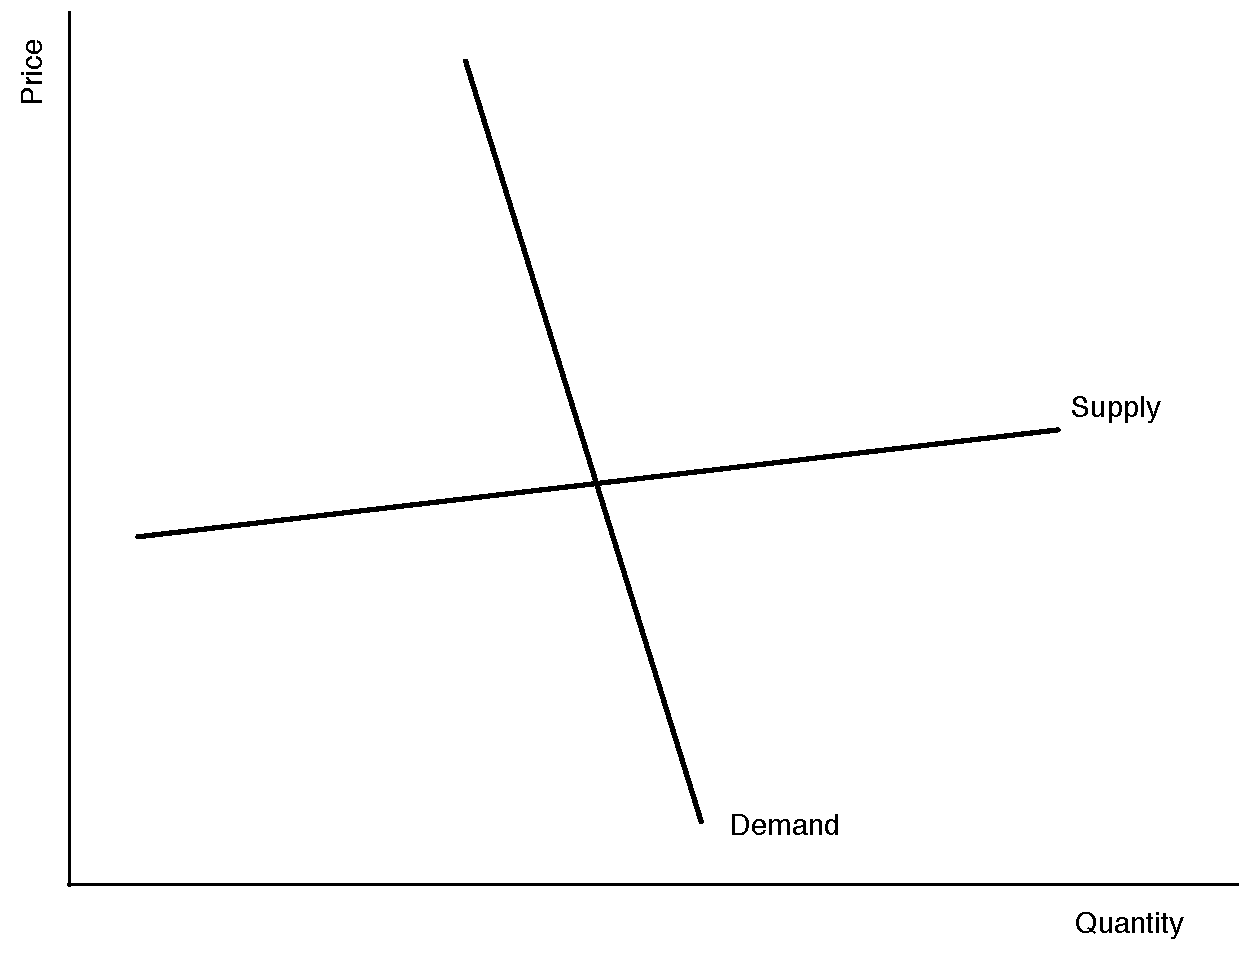
\includegraphics[scale=.45]{Exam1_MC19.pdf}
		\caption{Market for Coke}
		\label{fig1}
	\end{figure}
	
	If the government imposes a \$5 per unit tax on sellers in this market,  
	
	\begin{choices}
		\choice the burden of the tax will be split evenly between buyers and sellers in the market.
		\choice the burden of the tax will be greater for sellers than for buyers in the market.
		\CorrectChoice the burden of the tax will be greater for buyers than for sellers in the market.
		\choice the split of the tax burden cannot be determined from this information. 
	\end{choices}
	
	\begin{solution}
		Regardless of who the tax is levied against, the majority of the tax burden will fall on whoever has the more inelastic curve. From the graph, we see that demand is more inelastic and so buyers will bear a greater burden of the tax.
	\end{solution}
	

\uplevel{Refer to Figure \ref{fig2} for questions \ref{blah1} and \ref{blah2}.}

\begin{figure}[H]
	\centering
	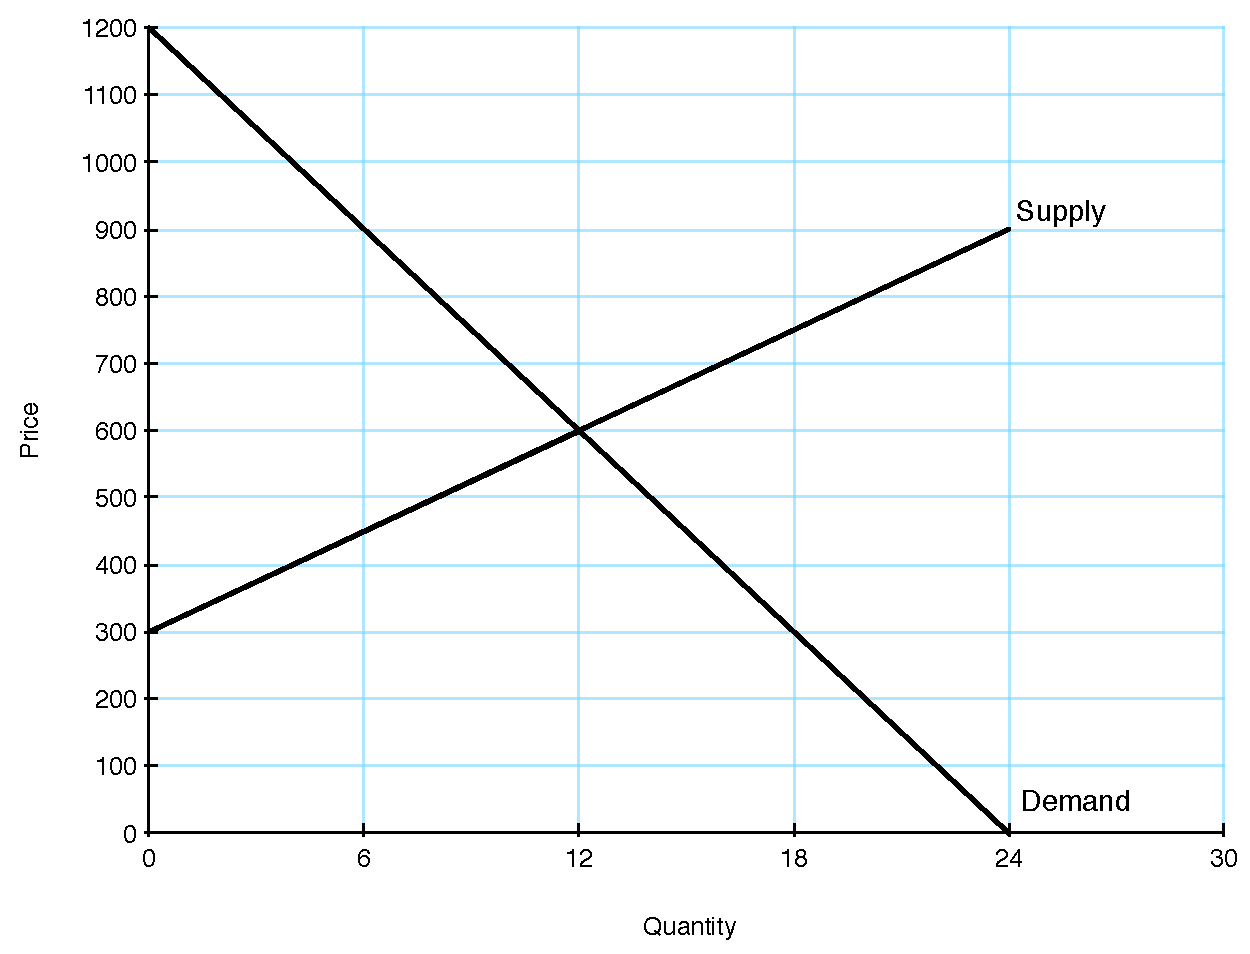
\includegraphics[scale=.45]{hw3_plot1.pdf}
	\caption{Market for Surface Tablets}
	\label{fig2}
\end{figure}

		
	\question \label{blah1} If the government imposes a price floor of \$900, then consumer surplus would \blank by \blank.
	
	\begin{choices}
		\choice increase; \$900
		\CorrectChoice decrease; \$2700
		\choice increase; \$2700
		\choice decrease; \$900
	\end{choices}
	
	\begin{solution}
		CS before the price floor is imposed is given area between the demand curve and $P^*$ = 600 up to $Q^*$ = 12. $CS_0$ = $1/2\cdot(600)\cdot(12) = \$3,600.$ CS after the price floor is imposed is given by area between the demand curve and $P_F$ = \$900 up to new quantity $Q_F$ = 6. $CS_1$ = $1/2 \cdot (300) \cdot (6) = \$900$. CS decreased by \$2,700.
	\end{solution}
	
	\question \label{blah2} As a result of this price floor, the total revenue earned by firms \blank because \blank.
	
	\begin{choices}
		\question increased; supply is inelastic 
		\question decreased; demand is inelastic
		\question increased; demand is inelastic
		\CorrectChoice decreased; demand is elastic
	\end{choices}
	
		
		\begin{solution}
			$TR_0 = P^* \times Q^* = \$600 \times 12 = \$7,200$. $TR_1 = P_F \times Q_F = \$900 \times 6 = \$5,400$. TR decreased, so it must be that demand is elastic between these points.
		\end{solution}
	
	
		\question A tax of \$4 is imposed by the government. Use Table \ref{MC27} to answer the question below.
		
		\begin{table}[H]
			\caption{Unit Taxes}
			\label{MC27}
			\centering
			\begin{tabular}{  c|c|c} 
				
				& Price with no tax & Price with \$4/unit tax on sellers \\
				\hline
				Price paid by buyers & \$55 & ? \\
				Price received by sellers & \$55 & \$53.50  \\
			\end{tabular}
		\end{table}
		
		Because of this tax, buyers are paying \underline{\hspace{3cm}} per unit and sellers are receiving \blank per unit.
		
		\begin{choices}
			\choice \$4 less; \$4 more
			\choice \$2 more; \$2 less
			\CorrectChoice \$2.50 more; \$1.50 less
			\choice \$4 more; \$4 less
		\end{choices}
		
		\begin{solution}
			Sellers receive \$55 - \$53.50 = \$1.50 less per unit. $P_B = P_S + \text{tax} = \$53.50 + \$4 = \$57.50 \Rightarrow$ buyers paying \$57.50 - \$55 = \$2.50 more than before.
		\end{solution}

	
	\question David's cat causes Carlos to sneeze. David values his cat's companionship at \$400 a year. Carlos has to pay for tissues and allergy medication due to the cat that cost him \$500 a year. According to the Coase Theorem,
	
	\begin{choices}
		\choice David should pay Carlos \$400 so he may keep his cat.
		\choice David should pay Carlos \$500 for his tissues and medication.
		\CorrectChoice Carlos should pay David \$410 to give away his cat.
		\choice None of the above.
	\end{choices}
	
	\begin{solution}
		David is willing to pay up to \$400 to Carlos to keep his cat, or he must receive more than \$400 in order to give his cat away. Carlos is willing to pay up to \$500 to David to get rid of the cat, or he must receive at least \$500 to be okay with it. Option C is the only one that works for both parties.
	\end{solution}
	
	
	\question If the production of a good yields a positive externality, then the social benefit curve lies \blank the demand curve, and the socially optimal quantity is \blank the market equilibrium quantity.
	
	\begin{choices}
		\CorrectChoice above; greater
		\choice above; less
		\choice below; greater
		\choice below; less
	\end{choices}
	
	\begin{solution}
		See class notes.
	\end{solution}
	
	\question The market equilibrium is not efficient when the consumption of a good creates external costs, which cause social costs to be 
	
	\begin{choices}
		\choice less than the private cost.
		\CorrectChoice greater than the private cost.
		\choice less than the total cost.
		\choice greater than the total cost.
	\end{choices}
	
	\begin{solution} 
		Social cost = private cost + external cost.
	\end{solution}


\question In the absence of intervention, negative externalities lead markets to produce

\begin{choices}
	\choice efficient output levels, and positive externalities lead markets to produce greater than efficient output levels.
	\choice smaller than efficient output levels, and positive externalities lead markets to produce greater than efficient output levels.
	\CorrectChoice greater than efficient output levels, and positive externalities lead markets to produce smaller than efficient output levels.
	\choice greater than efficient output levels, and positive externalities lead markets to produce efficient output levels.
\end{choices}

\begin{solution}
See class notes.
\end{solution}

\newpage

\question In order to eliminate the deadweight losses associated with a negative market externality, the government should impose a per unit tax \blank.
\begin{choices}
	\choice equal to the total external cost
	\choice less than the total external cost
	\choice greater than the per unit external cost.
	\CorrectChoice equal to the per unit external cost.
	\choice None of the above.
\end{choices}

\begin{solution}
	See class notes.
\end{solution}
	
	\question Which of following is an example of a common resource?
	
	\begin{choices}
		\choice Residential housing
		\choice National defense 
		\choice Restaurant meals
		\CorrectChoice Fish in the ocean
	\end{choices}
	
	\begin{solution}
		Common resources are non-excludable and rival. Housing and meals are rival and excludable. National defense in non-excludable and non-rival.
	\end{solution}

	
	\question A neighborhood street is considering purchasing and installing doggy clean up stations in order to keep their lawns clean. Table \ref{MC15} shows the willingness to pay of each family for each additional station.
	
	\begin{table}[H]
		\caption{Willingness to Pay for Doggy Stations}
		\label{MC15}
		\centering
		\begin{tabular}{ c|c|c|c} 
			
			Stations & Weiners Family & George Family & Heron Family\\
			\hline
			1st station & \$500 & \$600 & \$400\\
			2nd station & 400 & 450 & 300\\
			3rd station & 300 & 350 & 150\\
			4th station & 150 & 200 & 50\\
			5th station & 100 & 150 & 0\\
		\end{tabular}
	\end{table}
	
	If each doggy station costs \$500, how many stations should the street install in order to maximize total surplus?
	
	\begin{choices}
		\choice 2 stations
		\choice 0 stations
		\CorrectChoice 3 stations
		\choice 1 stations
		\choice > 3 stations
	\end{choices}

	\begin{solution}
		See example from class notes. Should build the station as long as the total WTP $\ge$ price/station.
	\end{solution}

		\question Public goods are 
		
		\begin{choices}
			\choice efficiently provided by market forces.
			\CorrectChoice underprovided in the absence of government.
			\choice overused in the absence of government.
			\choice a type of natural monopoly.
		\end{choices}
		
		\begin{solution}
			See class notes.
		\end{solution}
		
\newpage
		
	\question Which of the following examples demonstrates the free rider problem?
	\begin{choices}
		
		\CorrectChoice Josh downloads the podcast \textit{Serial}, but never contributes to NPR, its producer.
		\choice Liz Lemon is upset that she and Jack Donaghy pay the same amount at the toll booth, even though she only uses the road for 5 miles, while he uses it for 25 miles.
		\choice Due to a lack of clearly defined property rights, ocean creatures tend to be overfished.
		\choice Kristina, Jane, and Andrea rent three movies and enforce that the costs are split evenly, even though Jane is only willing to pay her share for two movies.
	\end{choices}
	
	\begin{solution}
		Free riders enjoy benefits without having to pay. In (b) Liz and Jack pay, (c) demonstrates issues with common resources, and (d) illustrates a forced rider.
	\end{solution}
		
		\question AJ opens a lemonade stand for two hours. He spends \$10 for ingredients and sells \$60 worth of lemonade. In those same two hours, he could have cleaned his neighbor's pool for \$40. AJ has an accounting profit of \blank and an economic profit of \blank.
		
		\begin{choices}
			\CorrectChoice \$50; \$10
			\choice \$90; \$50
			\choice \$10; \$50
			\choice \$50; \$90
		\end{choices}
		
		\begin{solution}
			Total revenue = \$60. Explicit costs = \$10. Implicit costs = \$40. Accounting profit = TR -- explicit costs = \$50. Economic profit = TR -- (explicit costs + implicit costs) = \$10.
		\end{solution}
		
		\question A firm is producing 100 units with an average total cost of \$25 and a marginal cost of \$15. If it were to increase production to 101 units, which of the following must occur?
		
		\begin{choices}
			\choice Marginal cost would decrease.
			\choice Marginal cost would increase.
			\CorrectChoice Average total cost would decrease.
			\choice Average total cost would increase.
		\end{choices}
		
		\begin{solution}
			If $MC < ATC$, then it must be that $ATC$ are decreasing.
		\end{solution}
		
	\question Bluth's Bananas currently employs 5 workers and produces 1,000 frozen bananas a day. In preparation for the busy summer season, the firm is debating whether they should hire 5 more workers. If they do, they project they could produce 1,500 frozen bananas a day. Given this, the marginal product of labor per worker from these additional workers would be
			
			\begin{choices}
				\choice 1,500.
				\choice 500.
				\choice 150.
				\CorrectChoice 100.
			\end{choices}
			
		\begin{solution}
			$MP_L = \frac{\Delta Q}{\Delta L} = \frac{(1,500 - 1,000)}{5} = 100.$
		\end{solution}

		\question Shell Tires has fixed costs of \$300,000 per year. Last year, it produced 10,000 tires with an average variable cost of \$80. What were the firm's average total costs for last year?
		
		\begin{choices}
			\choice \$80
			\choice \$90
			\choice \$100
			\CorrectChoice \$110
		\end{choices}
		
		\begin{solution}
			$ATC = TC/Q = (FC + VC)/Q = AFC + AVC = \$300,000/10,000 + \$80 = \$110$.
		\end{solution}

\newpage
		
		\question Keystone Fireworks has fixed costs of \$100 and the marginal costs outlined in Table \ref{tab1}.
		
		\begin{table}[H]
			\caption{Marginal Costs for Keystone}
			\label{tab1}
			\centering
		%Change last column to "H" for solutions
		\begin{tabular}{ c|c H}      
				Quantity & Marginal Cost & \dd{Variable Costs}\\     
				\hline
				1 & \$2 & \dd{\$2} \\
				2 & \$4 & \dd{\$6} \\
				3 & \$6 & \dd{\$12}\\
				4 & \$8 & \dd{\$20}  \\
				5 & \$10 & \dd{\$30} \\
				6 & \$12 & \dd{\$42}\\
			\end{tabular}
		\end{table}
		
		What is the average variable cost of producing the fifth unit?
		
		\begin{choices}
			\choice \$2
			\CorrectChoice \$6
			\choice \$10
			\choice \$30
		\end{choices}
		
		\begin{solution}
			At Q=0, VC = \$0. At Q=1, MC = \$2 which means VC increased by \$2 when going from Q=0 to Q=1. So, at Q=1, VC = \$2. At Q=2, MC = \$4, so VC increased by \$4 when going from Q=1 to Q=2. Since VC=\$2 at Q=1, at Q=2 VC =\$6. Continuing this process until Q=5, we have that VC = \$30. AVC = VC/Q = \$30/5 = \$6.
		\end{solution}
		
			\question A firm currently produces 1,000 units of output with an average variable cost of \$5.10. The firm has fixed costs of \$5,000. If the firm were to produce 1,001 units, its total variable costs would be \$5,400. What is the marginal cost to the firm of producing 1,001 units?
			
			\begin{choices}
				\choice \$5,400
				\CorrectChoice \$300
				\choice \$5,100
				\choice \$400
			\end{choices}
				
	\dd{At 1,000 units, $VC = 1,000 \times 5.10 = \$5,100.$ $MC = \frac{\Delta VC}{\Delta Q} = \frac{(5,400 - 5,100)}{1} = \$300.$}
		
\end{questions}

\subsection*{Short Answer}

\begin{questions}


	\question Consider public policy aimed at smoking.
	
		\begin{parts}
			\part[4] Studies indicate the price elasticity of demand for cigarettes is about 0.4. If a pack of smokes currently costs \$2 and the government wants to reduce smoking by 20\%, by how much should it increase the price (in percentage terms)? 
			
			\begin{solution}
				$\varepsilon_d^P = \frac{\%\Delta Q_d}{\%\Delta P} = -.4 \Rightarrow \frac{-20\%}{\%\Delta P} = -.4 \Rightarrow \%\Delta P = +50\%.$ The government should increase cigarette prices by 50\%. You can also use the elasticity formula to show that the new price should be \$3.33.
			\end{solution}
			
			\part[4] If the government permanently increases the price of cigarettes, will the policy have a larger effect on smoking one year from now or five years from now? Draw a graph to support your answer. 
			
			\begin{solution}
				See Figure \ref{fig3}. Demand in the short run is inelastic, and thus the quantity demanded will not decrease much due to the higher price. In the long run, demand becomes more elastic and thus the quantity demanded will fall more.
			
			
			
			\begin{figure}[H]
				\centering
				\includegraphics[scale=.35]{hw3_plot2.pdf}
				\caption{Demand for Cigarettes in SR and LR}
				\label{fig3}
			\end{figure}
			
			\end{solution}
			
			\part[2] Studies also find that teens have a higher price elasticity of demand than do adults. Why might this be true?
			
			\begin{solution}
				One of the determinants price elasticity of demand is whether a good is viewed as a luxury or a necessity. Adult smokers likely view cigarettes as more of a necessity than teens since they have been smoking for a longer amount of time and thus likely find it harder to quit. Therefore, the price elasticity of demand is likely higher for teens. Additionally, cigarettes likely consume a greater amount of the budget for teens than adults, and again this implies teens have a more elastic demand.
			\end{solution}
			
		\end{parts}
	
		\question Let's return to our study of the minimum wage.
		
		\begin{parts}
			
			\part[4] Suppose the minimum wage is above the market equilibrium wage in the market for unskilled labor. Draw a supply-and-demand diagram showing the market wage, the number of workers that are employed, and the number of workers who are unemployed. Also show the total wage payments to unskilled workers. \textbf{Hint:} We did this in class.
		
			\begin{solution}
				See Figure \ref{fig4}. 
			\end{solution}
			
			\part[4] What would be the effect of an increase in the minimum wage on employment? Does this change depend on the elasticity of demand, supply, both, or neither? Use a graph to support your answer. 
			
			\begin{solution}
				An increase in the minimum wage will lead to a decrease in the quantity of workers employed ($Q_{E1} \rightarrow Q_{E2}$ in the graph). This quantity depends on the elasticity of demand, as both points are on the demand curve.
			\end{solution}
			
			\part[4] What would be the effect of an increase in the minimum wage on unemployment? Does this change depend on the elasticity of demand, supply, both, or neither? Use a graph to support your answer. 
			
			\begin{solution}
				An increase in the minimum wage will lead to an increase in unemployment (unemployment 1 $\rightarrow$ unemployment 2 in the graph), as the quantity demanded decreases and quantity supplied increases. The change depends on the elasticity of both demand and supply.
			\end{solution}
			
			\part[2] Now consider the effect of an increase in the minimum wage on wage payments. What would happen to total wage payments if the demand for unskilled labor was inelastic? How does the elasticity of labor supply impact wage payments? \textbf{Hint:} Total wage payments are equivalent to the notion of total revenue in other markets we have studied.
			
			\begin{solution}
				With inelastic labor demand, total wage payments will increase with an increase in wages, as the increase in wages offsets the decrease in the number of workers employed. The elasticity of labor supply has no effect on $Q_E$, and so has no effect on total wage payments.
			\end{solution}
			
		\end{parts}
		
		\dd{
		\begin{figure}[H]
			\centering
			\includegraphics[scale=.45]{hw3_plot3.pdf}
			\caption{Labor Market with Minimum Wage}
			\label{fig4}
		\end{figure}}
		
		\question The many identical residents of Salisbury love drinking Cheerwine. Each resident has a certain willingness to pay for each can they consume as shown in Table \ref{tab3}.
	
		\begin{table}[H]
			\caption{WTP for Cheerwine}
			\label{tab3}
			\centering
			\begin{tabular}{ c|c} 
				Can & WTP \\       
				\hline
				1st can & \$5 \\
				2nd can & \$4 \\
				3rd can & \$3 \\
				4th can & \$2 \\
				5th can & \$1 \\
				>5 cans & \$0 \\
			\end{tabular}
		\end{table}
		
		\begin{parts}
			\part[4] The cost of producing Cheerwine is \$1.50. The competitive suppliers sell at this price and have a perfectly elastic supply curve. How many cans will each person consume? What is the total surplus per person in this market? 
			
			\begin{solution}
				Consumers purchase Cheerwine as long as their WTP $\ge$ \$1.50 $\Rightarrow Q_D = 4$/person. PS = \$0 if supply is perfectly elastic, so TS = CS = WTP -- P for each can purchased $\Rightarrow \text{TS} = (\$5 - 1.50) + (\$4 - 1.50) + (\$3-1.50) + (\$2 - 1.50) = \$8/\text{person}$.
			\end{solution}
			
			\part[4] Producing Cheerwine creates pollution. Each can has an external cost of \$1. Taking this additional cost into account, what is the total surplus per person?
			
			\begin{solution}
				Each can consumed has an external cost of \$1. If each citizen buys four cans, the total external cost/person = \$1/can $\times$ 4 cans/person = \$4/person. TS/person = \$8 - \$4 = \$4.
			\end{solution}
			
			\part[4] Mayor Woodson imposes a \$1 tax on Cheerwine. What is the consumption per person now? Calculate consumer surplus, the external cost, government revenue, and total surplus per person. 
			
			\begin{solution}
				Since supply is perfectly elastic, the entire burden of the tax will be borne by consumers, so the new price consumers pay is \$1.50 + \$1 = \$2.50. Consumers will each only buy 3 cans of Cheerwine now and \\\\
				 TS/person = $\underbrace{(\$5 - 2.50) + (\$4 - 2.50) + (\$3 - 2.50)}_{\text{Consumer surplus/person}} - \underbrace{\$1 \times 3}_{\text{TEC/person}} + \underbrace{\$1 \times 3}_{\text{Tax revenue}} = \$4.50$.\\\\
			By internalizing the externality, we got rid of the DWL and increased TS.
			\end{solution}
			
		\end{parts}
			
		\question[4] Your roommate's food truck sells delicious burritos every Friday night. He tells you a story that as he closed up shop last weekend, an inebriated patron yelled at him to make him one for \$10.00. Your roommate had already sold 200 burritos that night, but usually has to sell them for \$4.00 due to market conditions. He tells you that he obviously sold him the burrito for \$10.00. If he faces the cost schedule detailed in Table \ref{tab5}, was this the right decision? Explain why or why not. 
			
			
			\begin{table}[H]
				\caption{Burrito Costs}
				\centering
				\begin{tabular}{ c|c}        
					
					Quantity  & ATC \\
					\hline
					199 & \$1.99 \\
					200 & \$2.00 \\
					201 & \$2.05 \\
				\end{tabular}
				\label{tab5}
			\end{table}
			
			\begin{solution}
				Your roommate should sell the burrito as long as $MR \ge MC$. $MR = \$4.$ At Q=200, $TC = \$2.00 \times 200 = \$400$ and at Q=201 $TC = \$2.05 \times 201 = \$412.05.$ $MC = 412.05 - 400 = \$12.05$. Your friend should not have the sold burrito for \$10, as he would actually decrease his profit for the day by \$2.05.
			\end{solution}
		
		
	\question What topics or questions gave you the most trouble on this homework assignment or the class material it encompassed? 
			
\end{questions}

\end{document}